% Options for packages loaded elsewhere
\PassOptionsToPackage{unicode}{hyperref}
\PassOptionsToPackage{hyphens}{url}
%
\documentclass[
  10pt,
  ignorenonframetext,
]{beamer}
\usepackage{pgfpages}
\setbeamertemplate{caption}[numbered]
\setbeamertemplate{caption label separator}{: }
\setbeamercolor{caption name}{fg=normal text.fg}
\beamertemplatenavigationsymbolsempty
% Prevent slide breaks in the middle of a paragraph
\widowpenalties 1 10000
\raggedbottom
\setbeamertemplate{part page}{
  \centering
  \begin{beamercolorbox}[sep=16pt,center]{part title}
    \usebeamerfont{part title}\insertpart\par
  \end{beamercolorbox}
}
\setbeamertemplate{section page}{
  \centering
  \begin{beamercolorbox}[sep=12pt,center]{part title}
    \usebeamerfont{section title}\insertsection\par
  \end{beamercolorbox}
}
\setbeamertemplate{subsection page}{
  \centering
  \begin{beamercolorbox}[sep=8pt,center]{part title}
    \usebeamerfont{subsection title}\insertsubsection\par
  \end{beamercolorbox}
}
\AtBeginPart{
  \frame{\partpage}
}
\AtBeginSection{
  \ifbibliography
  \else
    \frame{\sectionpage}
  \fi
}
\AtBeginSubsection{
  \frame{\subsectionpage}
}
\usepackage{amsmath,amssymb}
\usepackage{lmodern}
\usepackage{ifxetex,ifluatex}
\ifnum 0\ifxetex 1\fi\ifluatex 1\fi=0 % if pdftex
  \usepackage[T1]{fontenc}
  \usepackage[utf8]{inputenc}
  \usepackage{textcomp} % provide euro and other symbols
\else % if luatex or xetex
  \usepackage{unicode-math}
  \defaultfontfeatures{Scale=MatchLowercase}
  \defaultfontfeatures[\rmfamily]{Ligatures=TeX,Scale=1}
\fi
\usecolortheme{beaver}
% Use upquote if available, for straight quotes in verbatim environments
\IfFileExists{upquote.sty}{\usepackage{upquote}}{}
\IfFileExists{microtype.sty}{% use microtype if available
  \usepackage[]{microtype}
  \UseMicrotypeSet[protrusion]{basicmath} % disable protrusion for tt fonts
}{}
\makeatletter
\@ifundefined{KOMAClassName}{% if non-KOMA class
  \IfFileExists{parskip.sty}{%
    \usepackage{parskip}
  }{% else
    \setlength{\parindent}{0pt}
    \setlength{\parskip}{6pt plus 2pt minus 1pt}}
}{% if KOMA class
  \KOMAoptions{parskip=half}}
\makeatother
\usepackage{xcolor}
\IfFileExists{xurl.sty}{\usepackage{xurl}}{} % add URL line breaks if available
\IfFileExists{bookmark.sty}{\usepackage{bookmark}}{\usepackage{hyperref}}
\hypersetup{
  pdftitle={Manejo de datos en R (II)},
  pdfauthor={Introducción a la Línea de Comandos para Análisis Bioinformáticos},
  hidelinks,
  pdfcreator={LaTeX via pandoc}}
\urlstyle{same} % disable monospaced font for URLs
\newif\ifbibliography
\usepackage{color}
\usepackage{fancyvrb}
\newcommand{\VerbBar}{|}
\newcommand{\VERB}{\Verb[commandchars=\\\{\}]}
\DefineVerbatimEnvironment{Highlighting}{Verbatim}{commandchars=\\\{\}}
% Add ',fontsize=\small' for more characters per line
\usepackage{framed}
\definecolor{shadecolor}{RGB}{248,248,248}
\newenvironment{Shaded}{\begin{snugshade}}{\end{snugshade}}
\newcommand{\AlertTok}[1]{\textcolor[rgb]{0.94,0.16,0.16}{#1}}
\newcommand{\AnnotationTok}[1]{\textcolor[rgb]{0.56,0.35,0.01}{\textbf{\textit{#1}}}}
\newcommand{\AttributeTok}[1]{\textcolor[rgb]{0.77,0.63,0.00}{#1}}
\newcommand{\BaseNTok}[1]{\textcolor[rgb]{0.00,0.00,0.81}{#1}}
\newcommand{\BuiltInTok}[1]{#1}
\newcommand{\CharTok}[1]{\textcolor[rgb]{0.31,0.60,0.02}{#1}}
\newcommand{\CommentTok}[1]{\textcolor[rgb]{0.56,0.35,0.01}{\textit{#1}}}
\newcommand{\CommentVarTok}[1]{\textcolor[rgb]{0.56,0.35,0.01}{\textbf{\textit{#1}}}}
\newcommand{\ConstantTok}[1]{\textcolor[rgb]{0.00,0.00,0.00}{#1}}
\newcommand{\ControlFlowTok}[1]{\textcolor[rgb]{0.13,0.29,0.53}{\textbf{#1}}}
\newcommand{\DataTypeTok}[1]{\textcolor[rgb]{0.13,0.29,0.53}{#1}}
\newcommand{\DecValTok}[1]{\textcolor[rgb]{0.00,0.00,0.81}{#1}}
\newcommand{\DocumentationTok}[1]{\textcolor[rgb]{0.56,0.35,0.01}{\textbf{\textit{#1}}}}
\newcommand{\ErrorTok}[1]{\textcolor[rgb]{0.64,0.00,0.00}{\textbf{#1}}}
\newcommand{\ExtensionTok}[1]{#1}
\newcommand{\FloatTok}[1]{\textcolor[rgb]{0.00,0.00,0.81}{#1}}
\newcommand{\FunctionTok}[1]{\textcolor[rgb]{0.00,0.00,0.00}{#1}}
\newcommand{\ImportTok}[1]{#1}
\newcommand{\InformationTok}[1]{\textcolor[rgb]{0.56,0.35,0.01}{\textbf{\textit{#1}}}}
\newcommand{\KeywordTok}[1]{\textcolor[rgb]{0.13,0.29,0.53}{\textbf{#1}}}
\newcommand{\NormalTok}[1]{#1}
\newcommand{\OperatorTok}[1]{\textcolor[rgb]{0.81,0.36,0.00}{\textbf{#1}}}
\newcommand{\OtherTok}[1]{\textcolor[rgb]{0.56,0.35,0.01}{#1}}
\newcommand{\PreprocessorTok}[1]{\textcolor[rgb]{0.56,0.35,0.01}{\textit{#1}}}
\newcommand{\RegionMarkerTok}[1]{#1}
\newcommand{\SpecialCharTok}[1]{\textcolor[rgb]{0.00,0.00,0.00}{#1}}
\newcommand{\SpecialStringTok}[1]{\textcolor[rgb]{0.31,0.60,0.02}{#1}}
\newcommand{\StringTok}[1]{\textcolor[rgb]{0.31,0.60,0.02}{#1}}
\newcommand{\VariableTok}[1]{\textcolor[rgb]{0.00,0.00,0.00}{#1}}
\newcommand{\VerbatimStringTok}[1]{\textcolor[rgb]{0.31,0.60,0.02}{#1}}
\newcommand{\WarningTok}[1]{\textcolor[rgb]{0.56,0.35,0.01}{\textbf{\textit{#1}}}}
\usepackage{graphicx}
\makeatletter
\def\maxwidth{\ifdim\Gin@nat@width>\linewidth\linewidth\else\Gin@nat@width\fi}
\def\maxheight{\ifdim\Gin@nat@height>\textheight\textheight\else\Gin@nat@height\fi}
\makeatother
% Scale images if necessary, so that they will not overflow the page
% margins by default, and it is still possible to overwrite the defaults
% using explicit options in \includegraphics[width, height, ...]{}
\setkeys{Gin}{width=\maxwidth,height=\maxheight,keepaspectratio}
% Set default figure placement to htbp
\makeatletter
\def\fps@figure{htbp}
\makeatother
\setlength{\emergencystretch}{3em} % prevent overfull lines
\providecommand{\tightlist}{%
  \setlength{\itemsep}{0pt}\setlength{\parskip}{0pt}}
\setcounter{secnumdepth}{-\maxdimen} % remove section numbering
\usepackage{tikz}
\usepackage{graphicx}
\usetikzlibrary{calc}
\usepackage{pgfplots}
\usepackage{ragged2e}
\usepackage{svg}
\usepackage{environ}
\useoutertheme{miniframes}
\useinnertheme{circles}
\ifluatex
  \usepackage{selnolig}  % disable illegal ligatures
\fi

\title{Manejo de datos en R (II)}
\author{Introducción a la Línea de Comandos para Análisis
Bioinformáticos}
\date{11 de Agosto, 2021}

\begin{document}
\frame{\titlepage}

\hypertarget{breve-repaso}{%
\section{Breve repaso}\label{breve-repaso}}

\begin{frame}{Algunas ventajas de usar \emph{R}}
\protect\hypertarget{algunas-ventajas-de-usar-r}{}
\begin{itemize}
\item
  Lenguaje potente pero de relativa facil entradac \vspace{10pt}
\item
  Buena integracion de:

  \begin{itemize}
  \tightlist
  \item
    importe de datos de diferente formato
  \item
    edicion y filtrado de datos
  \item
    visualizacion/modelado de datos (analisis exploratorio)
  \item
    comunicacion de resultados (RMarkdown)
  \end{itemize}
\end{itemize}

\vspace{10pt}

\begin{itemize}
\tightlist
\item
  Es particularmente popular en biologia computacional (especialmente
  eco-evo y genomicas) \vspace{10pt}
\item
  Queremos hacer graficos de alta calidad!
\end{itemize}
\end{frame}

\begin{frame}{Manejo de datos y análisis reproducible}
\protect\hypertarget{manejo-de-datos-y-anuxe1lisis-reproducible}{}
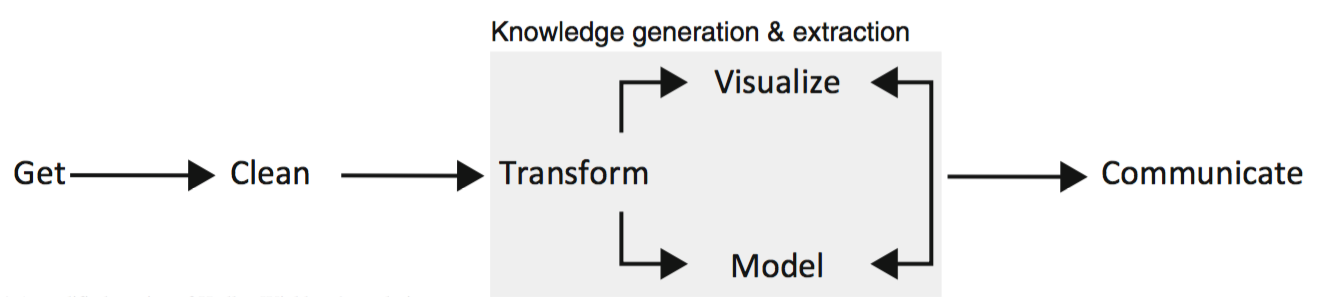
\includegraphics{../../imgs/analytic_process.png}

\vspace{60pt}

\raggedleft \small \href{http://93.174.95.29/_ads/6F902E466A32011DD94E2B6EEE505F9F}{Data
Wrangling with R (Boehmke, 2016)}
\end{frame}

\begin{frame}{Operaciones sobre datos}
\protect\hypertarget{operaciones-sobre-datos}{}
\begin{itemize}
\tightlist
\item
  Cargar datos \emph{crudos}/Guardar datos finales y tablas de interés.
  \vspace{10pt}
\item
  Filtrar datos (con criterio). \vspace{10pt}
\item
  Unir datos que vienen de diferentes fuentes, referentes a un mismo
  conjunto estudiado. \vspace{10pt}
\item
  Hacer modificaciones: crear \emph{tags}, correcciones ortográficas,
  filas y columnas de tablas, etc\ldots{} \vspace{10pt}
\item
  Generar nuevos datos: obtener promedios, medianas, aplicar funciones
  de librerías. \vspace{10pt}
\item
  Visualiar/modelar datos \vspace{10pt}
\item
  Dejar anotado y reportar lo hecho.
\end{itemize}
\end{frame}

\hypertarget{tidyverse-una-forma-de-programar-en-r}{%
\section{\texorpdfstring{\emph{tidyverse}: una forma de programar en
\emph{R}}{tidyverse: una forma de programar en R}}\label{tidyverse-una-forma-de-programar-en-r}}

\begin{frame}{}
\protect\hypertarget{section}{}
\begin{tikzpicture}[remember picture,overlay]
  \node[anchor=south west,inner sep=0pt] at ($(current page.south west)+(0cm,7.8cm)$) {
     
\includegraphics[width=1.5cm]{../../imgs/tidyverse.png}
  };
\end{tikzpicture}

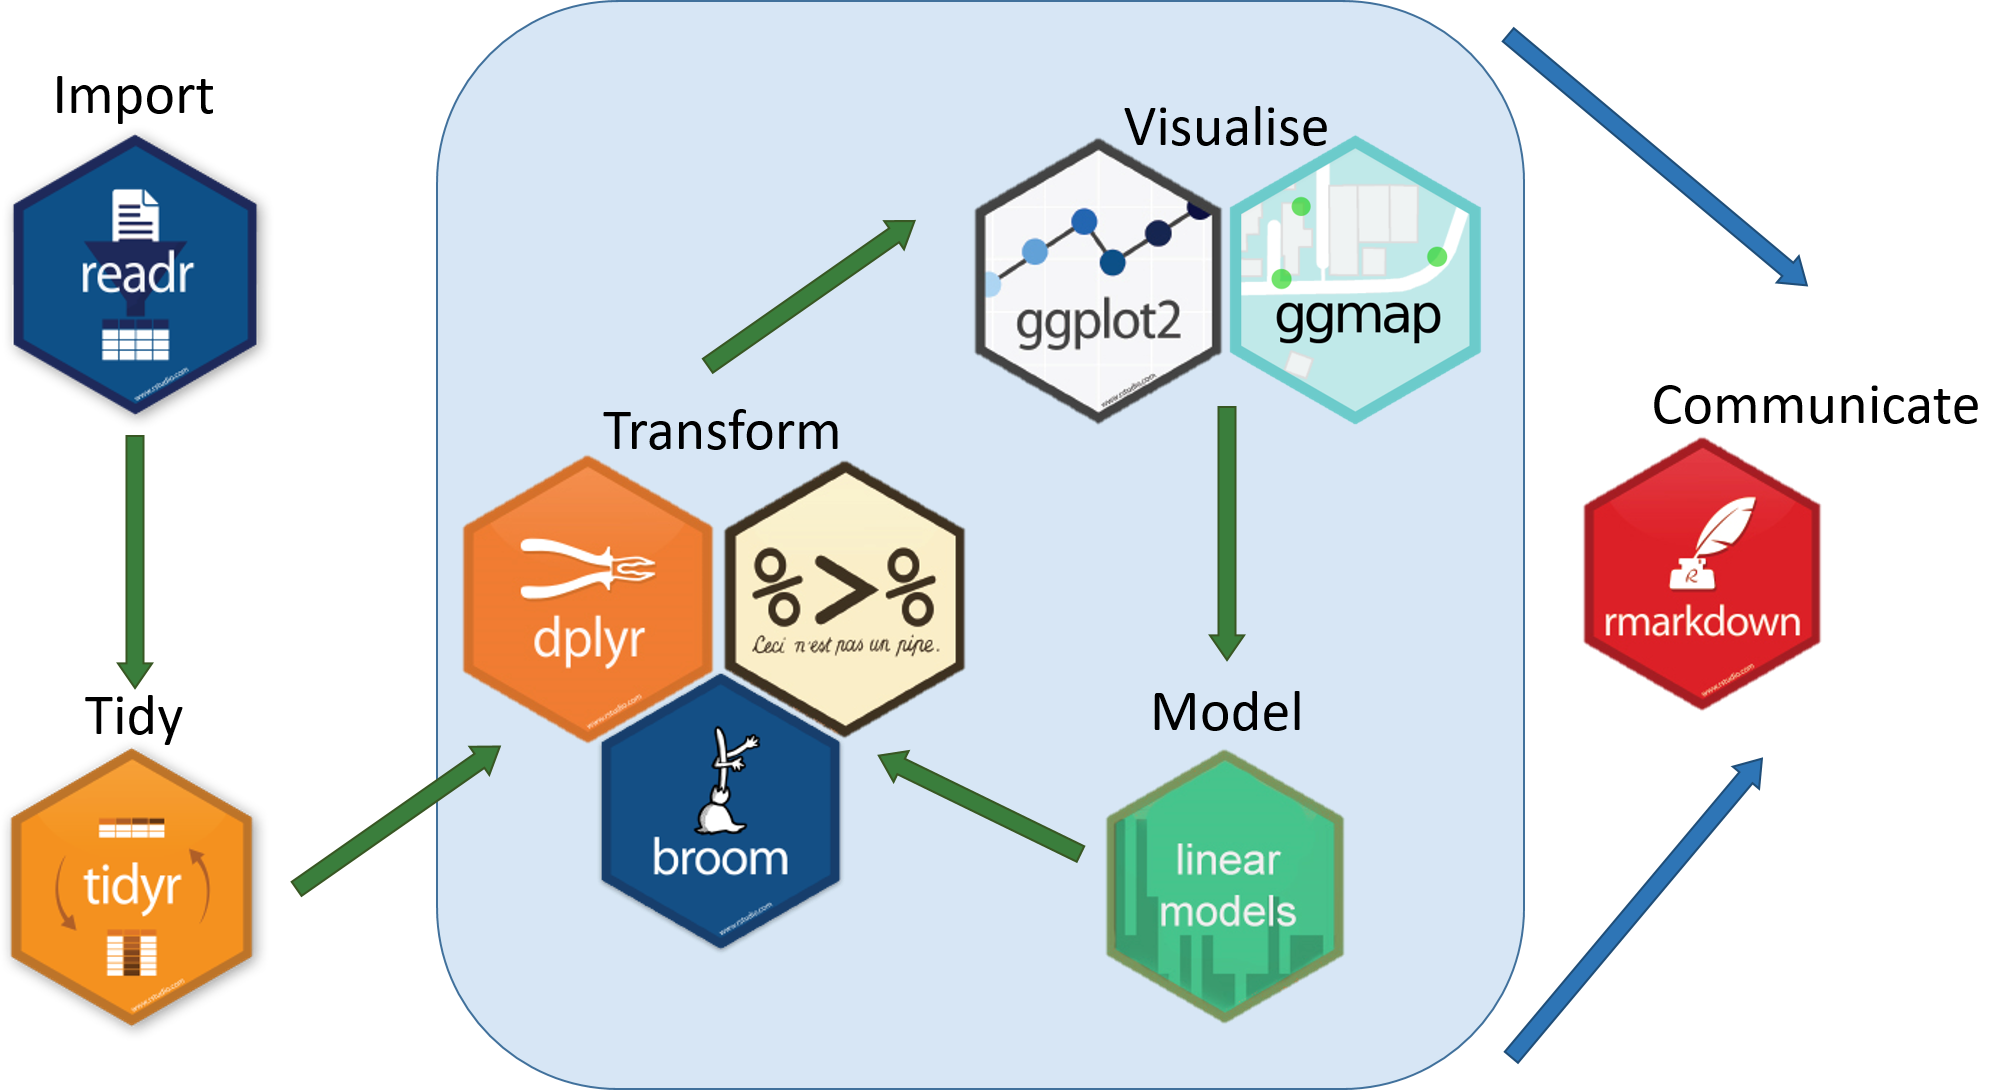
\includegraphics{../../imgs/tidyverse_packages.png}

\begin{itemize}
\tightlist
\item
  Hay librerias del universo \emph{tidyverse} para cada paso clave de
  analisis de datos.
\item
  Hay, ademas, librerias con su logica para analisis especificos:
  estadistica, modelado de datos, filogenetica, genomica, etc\ldots{}
\end{itemize}
\end{frame}

\begin{frame}{\emph{tidy} data}
\protect\hypertarget{tidy-data}{}
``\emph{Tidy}'' en ingles significa ``ordenado'', de ahi el nombre de la
libreria.

\begin{center}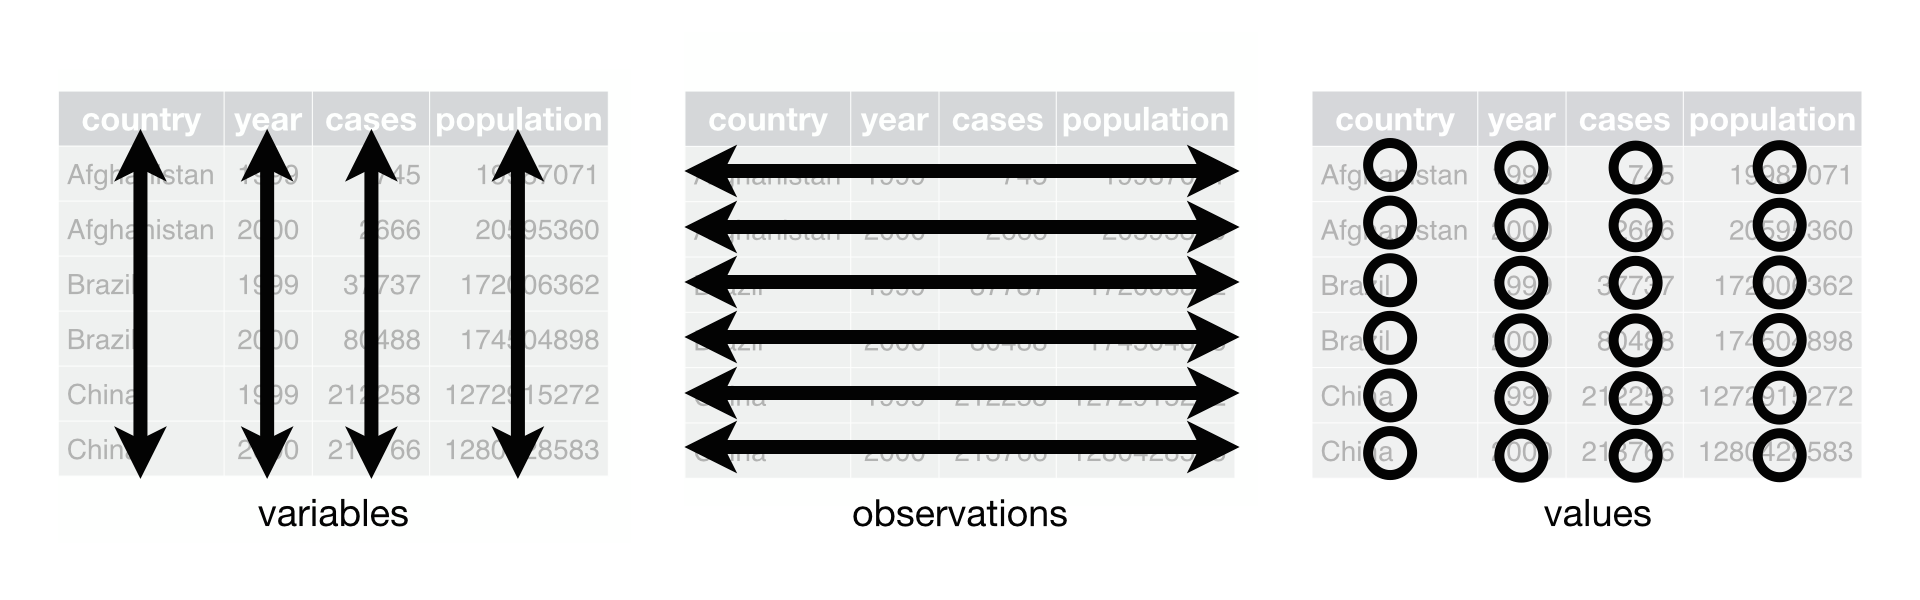
\includegraphics{../../imgs/tidy_data_specification} \end{center}

\begin{itemize}
\tightlist
\item
  Caracteristicas de \emph{tidy} data:

  \begin{itemize}
  \tightlist
  \item
    Cada fila corresponde a una observacion
  \item
    Cada columna corresponde a una variable
  \end{itemize}
\item
  \textbf{Ventajas}:

  \begin{itemize}
  \tightlist
  \item
    Estandarizacion
  \item
    Se basa, y le saca jugo, a la logica vectoria de \emph{R}
  \item
    Ya tenemos todos los paquetes de \emph{tidyverse} para trabajar
    arriba de la \emph{tidy} data! (y generarla).
  \end{itemize}
\end{itemize}
\end{frame}

\begin{frame}{Operaciones sobre datos (con \emph{tidyverse})}
\protect\hypertarget{operaciones-sobre-datos-con-tidyverse}{}
\begin{itemize}
\tightlist
\item
  Cargar datos \emph{crudos}/Guardar datos finales y tablas de interés.
  (\textbf{readr}) \vspace{10pt}
\item
  Filtrar datos (con criterio). (\textbf{dplyr}) \vspace{10pt}
\item
  dplyr.svg Unir datos que vienen de diferentes fuentes, referentes a un
  mismo conjunto estudiado. (\textbf{dplyr}) \vspace{10pt}
\item
  Hacer modificaciones: crear \emph{tags}, correcciones ortográficas,
  filas y columnas de tablas, etc\ldots{} (\textbf{tidyr}) \vspace{10pt}
\item
  magrittr\_logo.png dplyr.png Generar nuevos datos: obtener promedios,
  medianas, aplicar funciones de librerías. (\textbf{magrittr} +
  \textbf{dplyr}) \vspace{10pt}
\item
  Visualiar/modelar datos (\textbf{ggplot2} + \textbf{tidymodels})
  \vspace{10pt}
\item
  Dejar anotado y reportar lo hecho. (\textbf{rmarkdown},
  \textbf{blogdown})
\end{itemize}
\end{frame}

\begin{frame}[fragile]{}
\protect\hypertarget{section-1}{}
\begin{tikzpicture}[remember picture,overlay]
  \node[anchor=south west,inner sep=0pt] at ($(current page.south west)+(0cm,7.8cm)$) {
     
\includegraphics[width=1.5cm]{../../imgs/tibbles.png}
  };
\end{tikzpicture}

\scriptsize

\begin{Shaded}
\begin{Highlighting}[]
\FunctionTok{library}\NormalTok{(tibble)}

\FunctionTok{as\_tibble}\NormalTok{(iris)}
\end{Highlighting}
\end{Shaded}

\begin{verbatim}
## # A tibble: 150 x 5
##    Sepal.Length Sepal.Width Petal.Length Petal.Width Species
##           <dbl>       <dbl>        <dbl>       <dbl> <fct>  
##  1          5.1         3.5          1.4         0.2 setosa 
##  2          4.9         3            1.4         0.2 setosa 
##  3          4.7         3.2          1.3         0.2 setosa 
##  4          4.6         3.1          1.5         0.2 setosa 
##  5          5           3.6          1.4         0.2 setosa 
##  6          5.4         3.9          1.7         0.4 setosa 
##  7          4.6         3.4          1.4         0.3 setosa 
##  8          5           3.4          1.5         0.2 setosa 
##  9          4.4         2.9          1.4         0.2 setosa 
## 10          4.9         3.1          1.5         0.1 setosa 
## # ... with 140 more rows
\end{verbatim}

\normalsize

\begin{itemize}
\tightlist
\item
  En \emph{tidyverse} se suele trabajar sobre tablas en formato
  \emph{tidy}, alojadas en objetos de clase \textbf{tibble}
\item
  A las mismas se le aplican varios procesos
\end{itemize}
\end{frame}

\begin{frame}{}
\protect\hypertarget{section-2}{}
\begin{tikzpicture}[remember picture,overlay]
  \node[anchor=south west,inner sep=0pt] at ($(current page.south west)+(0cm,7.8cm)$) {
     
\includegraphics[width=1.5cm]{../../imgs/magrittr_log.jpg}
  };
\end{tikzpicture}

\begin{center}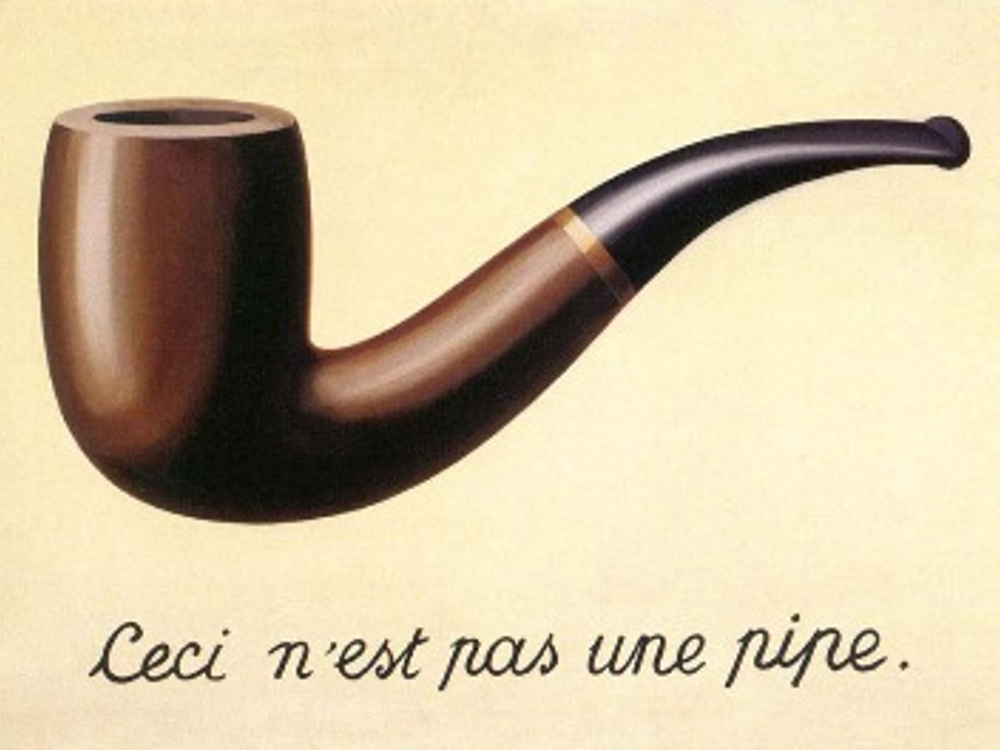
\includegraphics[height=0.6\textheight]{../../imgs/streamlining-with-magrittr} \end{center}

\begin{itemize}
\tightlist
\item
  Es el \emph{pipe} de R.
\item
  El uso es exactamente igual al `\textbar{}' de Bash.
\item
  Un único detalle: se utiliza \textbf{.} para hacer referencia a
  resultados intermedios en un pipe.
\end{itemize}
\end{frame}

\begin{frame}[fragile]{Operando secuencialmente sobre un dataset}
\protect\hypertarget{operando-secuencialmente-sobre-un-dataset}{}
\scriptsize

\begin{Shaded}
\begin{Highlighting}[]
\CommentTok{\# cargo las librerias que utilizamos en el practico}
\FunctionTok{library}\NormalTok{(magrittr)}
\FunctionTok{library}\NormalTok{(tidyverse)}

\CommentTok{\# cargo tabla CSV, separo datos de una columna y filtro datos de una columna}
\NormalTok{aeropuertos\_tibble }\OtherTok{=}\NormalTok{ readr}\SpecialCharTok{::}\FunctionTok{read\_csv}\NormalTok{(}\StringTok{\textquotesingle{}airport{-}codes.csv\textquotesingle{}}\NormalTok{) }\SpecialCharTok{\%\textgreater{}\%}
\NormalTok{  tidyr}\SpecialCharTok{::}\FunctionTok{separate}\NormalTok{(}\AttributeTok{data =}\NormalTok{ ., }
                  \AttributeTok{col =} \StringTok{\textquotesingle{}coordinates\textquotesingle{}}\NormalTok{, }
                  \AttributeTok{into =} \FunctionTok{c}\NormalTok{(}\StringTok{\textquotesingle{}lon\textquotesingle{}}\NormalTok{, }\StringTok{\textquotesingle{}lat\textquotesingle{}}\NormalTok{), }
                  \AttributeTok{sep =} \StringTok{\textquotesingle{}, \textquotesingle{}}\NormalTok{) }\SpecialCharTok{\%\textgreater{}\%}
\NormalTok{  dplyr}\SpecialCharTok{::}\FunctionTok{filter}\NormalTok{(}\FunctionTok{is.na}\NormalTok{(iso\_country))}
\end{Highlighting}
\end{Shaded}

\normalsize

Esta logica secuencial es sumamente practica. Pueden verla en accion si
siguen
\href{https://rpubs.com/mlangleib/linea_comandos_practico_12}{este link
a clase de practico}, junto a otras utilidades de \emph{tidyverse}.
\end{frame}

\hypertarget{gramatica-de-graficos-en-capas}{%
\section{Gramatica de graficos en
capas}\label{gramatica-de-graficos-en-capas}}

\begin{frame}{}
\protect\hypertarget{section-3}{}
\begin{tikzpicture}[remember picture,overlay]
  \node[anchor=south west,inner sep=0pt] at ($(current page.south west)+(0cm,7.8cm)$) {
     
\includegraphics[width=1.5cm]{../../imgs/ggplot2_logo.png}
  };
\end{tikzpicture}

La idea central es que un grafico puede ser construido a traves de capas
de elementos.

\begin{center}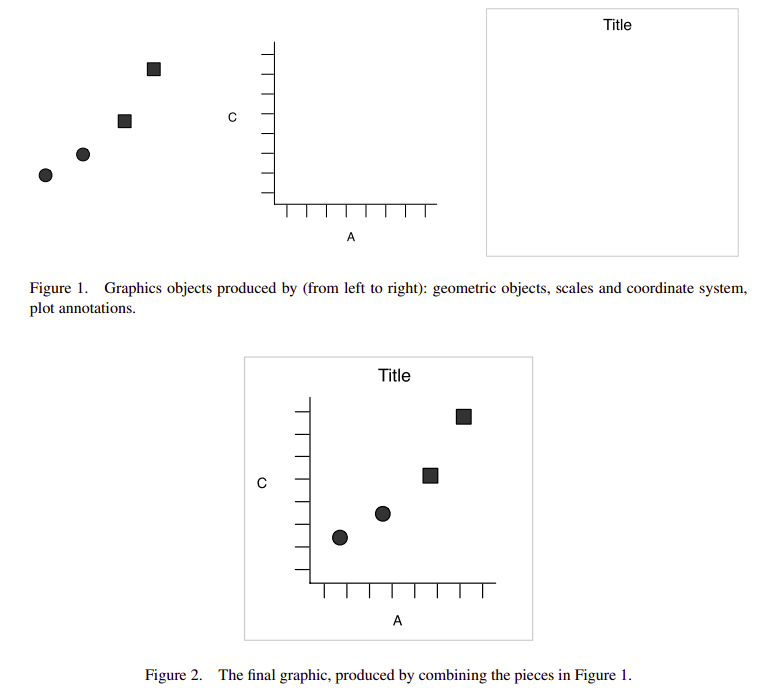
\includegraphics[width=0.72\linewidth]{../../imgs/logica_layered_grammar_of_graphics} \end{center}
\end{frame}

\begin{frame}{}
\protect\hypertarget{section-4}{}
\begin{tikzpicture}[remember picture,overlay]
  \node[anchor=south west,inner sep=0pt] at ($(current page.south west)+(0cm,7.8cm)$) {
     
\includegraphics[width=1.5cm]{../../imgs/ggplot2_logo.png}
  };
\end{tikzpicture}

La idea central es que un grafico puede ser construido a traves de capas
de elementos.

\begin{itemize}
\item
  Para realizar un gráfico preciso especificar:

  \begin{itemize}
  \tightlist
  \item
    Los \textbf{datos} sobre los que trabajo \vspace{10pt}
  \item
    Un sistema de coordenadas \vspace{10pt}
  \item
    Una especificación de qué representa cada dato a nivel
    \textbf{estético} \vspace{10pt}
  \item
    Una \textbf{forma geométrica} para representar estos datos
    \vspace{10pt}
  \end{itemize}
\item
  Además, podríamos considerar

  \begin{itemize}
  \tightlist
  \item
    Especificar \textbf{funciones} que operen sobre nuestros datos,
    agrupándolos o transformándolos (pasa en histogramas, por ejemplo)
    \vspace{10pt}
  \item
    \textbf{Subdivisiones} de nuestros datos en base a factores.
    \vspace{10pt}
  \end{itemize}
\end{itemize}
\end{frame}

\begin{frame}{}
\protect\hypertarget{section-5}{}
\begin{tikzpicture}[remember picture,overlay]
  \node[anchor=south west,inner sep=0pt] at ($(current page.south west)+(0cm,7.8cm)$) {
     
\includegraphics[width=1.5cm]{../../imgs/ggplot2_logo.png}
  };
\end{tikzpicture}

\begin{itemize}
\item
  Para realizar un gráfico preciso especificar:

  \begin{itemize}
  \tightlist
  \item
    Los \textbf{datos} sobre los que trabajo \(\rightarrow\) funcion
    \textbf{ggplot()} \vspace{10pt}
  \item
    Un sistema de coordenadas \(\rightarrow\) funcion \textbf{ggplot()}
    \vspace{10pt}
  \item
    Una especificación de qué representa cada dato a nivel
    \textbf{estético} \(\rightarrow\) funcion \textbf{aes()}
    \vspace{10pt}
  \item
    Una \textbf{forma geométrica} para representar estos datos funciones
    \(\rightarrow\) funciones \textbf{geom()}\_* \vspace{10pt}
  \end{itemize}
\item
  Además, podríamos considerar \vspace{10pt}

  \begin{itemize}
  \tightlist
  \item
    Especificar \textbf{funciones} que operen sobre nuestros datos,
    agrupándolos o transformándolos (pasa en histogramas, por ejemplo)
    \(\rightarrow\) funcion \textbf{stat()} \vspace{10pt}
  \item
    \textbf{Subdivisiones} de nuestros datos en base a factores.
    \(\rightarrow\) funcion \textbf{facet\_wrap}
  \end{itemize}
\end{itemize}
\end{frame}

\begin{frame}{}
\protect\hypertarget{section-6}{}
\begin{tikzpicture}[remember picture,overlay]
  \node[anchor=south west,inner sep=0pt] at ($(current page.south west)+(0cm,7.8cm)$) {
     
\includegraphics[width=1.5cm]{../../imgs/ggplot2_logo.png}
  };
\end{tikzpicture}

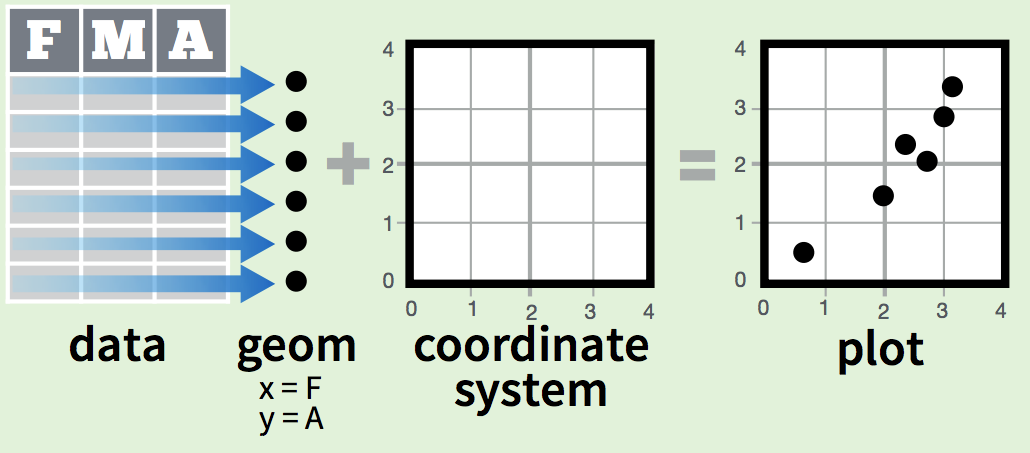
\includegraphics{../../imgs/ggplot_basico_1.png}
\end{frame}

\begin{frame}{}
\protect\hypertarget{section-7}{}
\begin{tikzpicture}[remember picture,overlay]
  \node[anchor=south west,inner sep=0pt] at ($(current page.south west)+(0cm,7.8cm)$) {
     
\includegraphics[width=1.5cm]{../../imgs/ggplot2_logo.png}
  };
\end{tikzpicture}

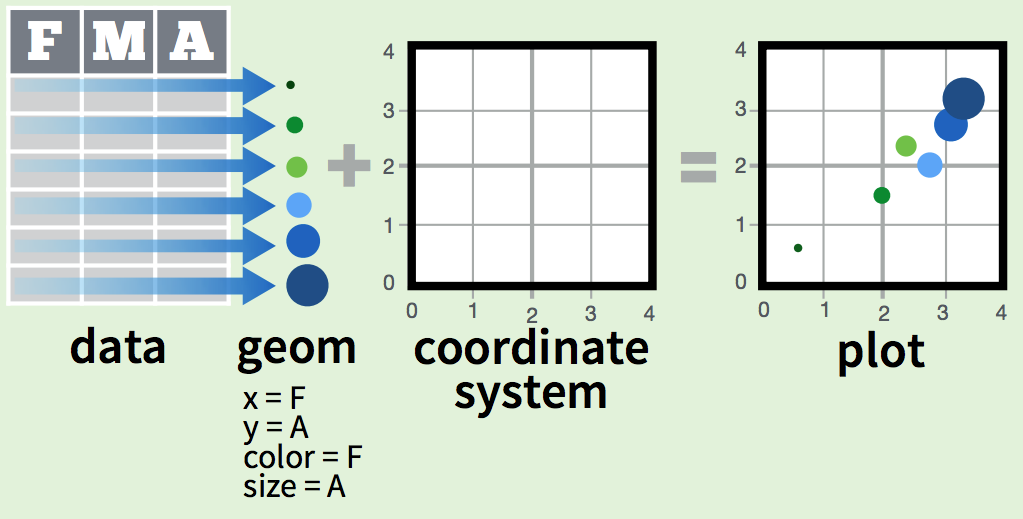
\includegraphics{../../imgs/ggplot_basico_2.png}
\end{frame}

\begin{frame}[fragile]{}
\protect\hypertarget{section-8}{}
\begin{tikzpicture}[remember picture,overlay]
  \node[anchor=south west,inner sep=0pt] at ($(current page.south west)+(0cm,7.8cm)$) {
     
\includegraphics[width=1.5cm]{../../imgs/ggplot2_logo.png}
  };
\end{tikzpicture}

\begin{Shaded}
\begin{Highlighting}[]
\FunctionTok{library}\NormalTok{(tidyverse)}
  \CommentTok{\# se grafica Sepal.Length vs Sepal.Width,}
  \CommentTok{\# coloreando segun Species}
\FunctionTok{ggplot}\NormalTok{(}\AttributeTok{data =}\NormalTok{ iris,}
       \AttributeTok{mapping =} \FunctionTok{aes}\NormalTok{(}\AttributeTok{x =}\NormalTok{ Sepal.Length, }
              \AttributeTok{y =}\NormalTok{ Sepal.Width, }
              \AttributeTok{color =}\NormalTok{ Species, }
              \AttributeTok{fill =}\NormalTok{ Species)) }\SpecialCharTok{+}
  \CommentTok{\# se grafica utilizando puntos}
  \FunctionTok{geom\_point}\NormalTok{() }
\end{Highlighting}
\end{Shaded}
\end{frame}

\begin{frame}{}
\protect\hypertarget{section-9}{}
\begin{tikzpicture}[remember picture,overlay]
  \node[anchor=south west,inner sep=0pt] at ($(current page.south west)+(0cm,7.8cm)$) {
     
\includegraphics[width=1.5cm]{../../imgs/ggplot2_logo.png}
  };
\end{tikzpicture}

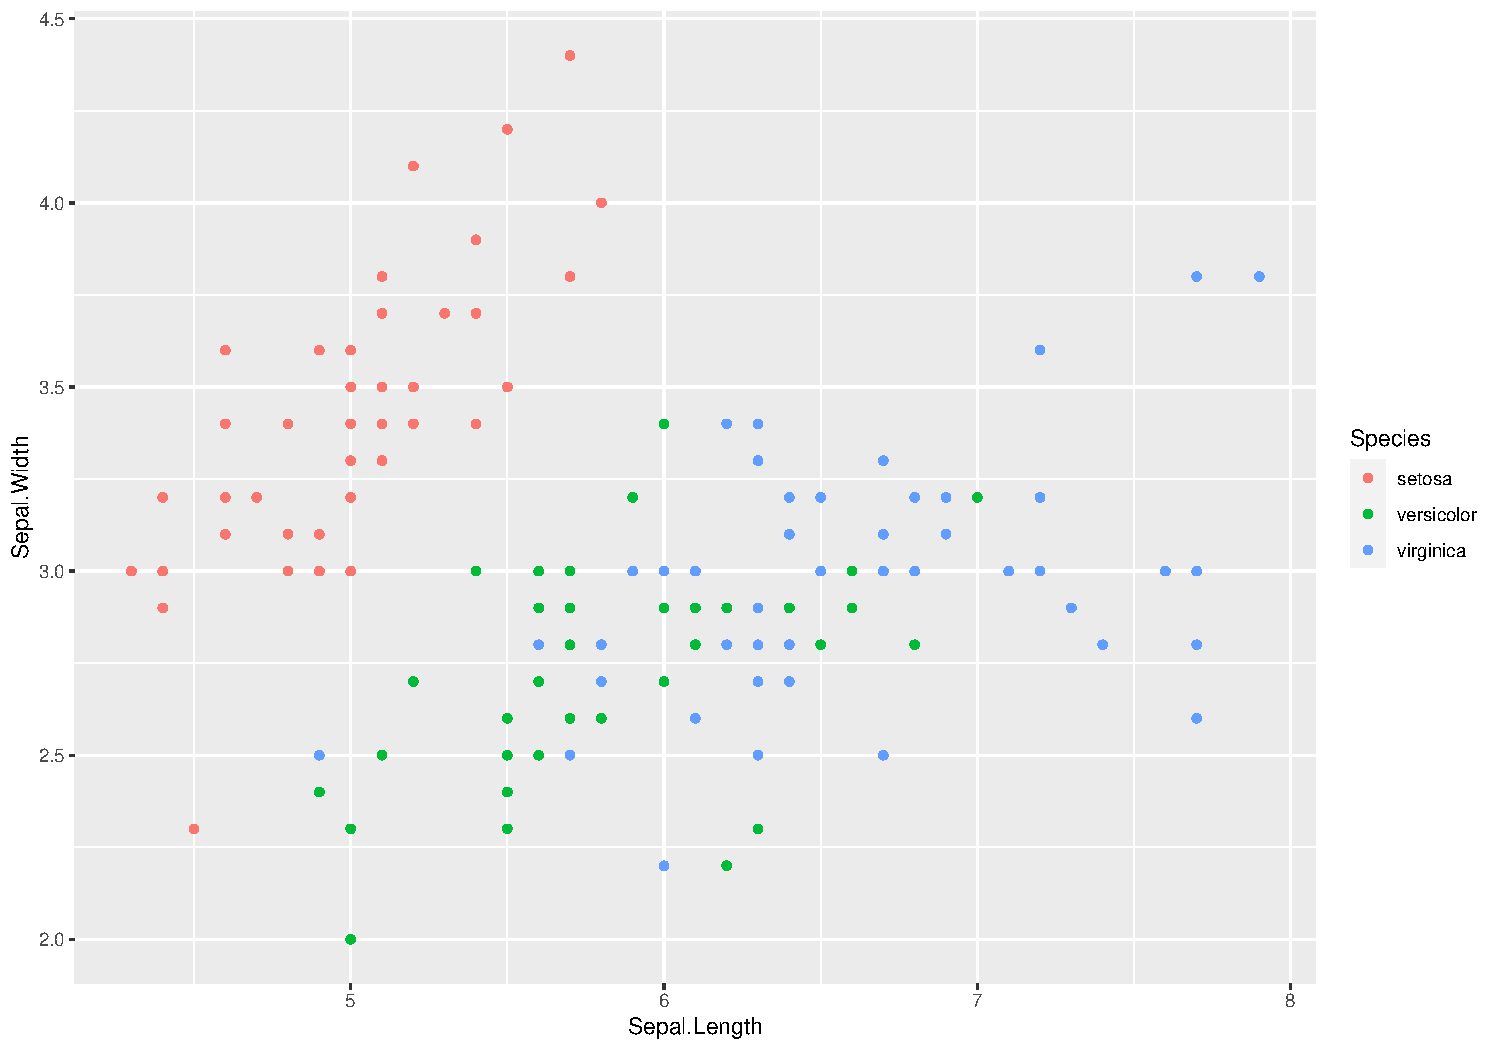
\includegraphics{claseIntro_practico12_final_files/figure-beamer/unnamed-chunk-18-1.pdf}
\end{frame}

\begin{frame}{GGally: análisis exploratorios y otros}
\protect\hypertarget{ggally-anuxe1lisis-exploratorios-y-otros}{}
\small

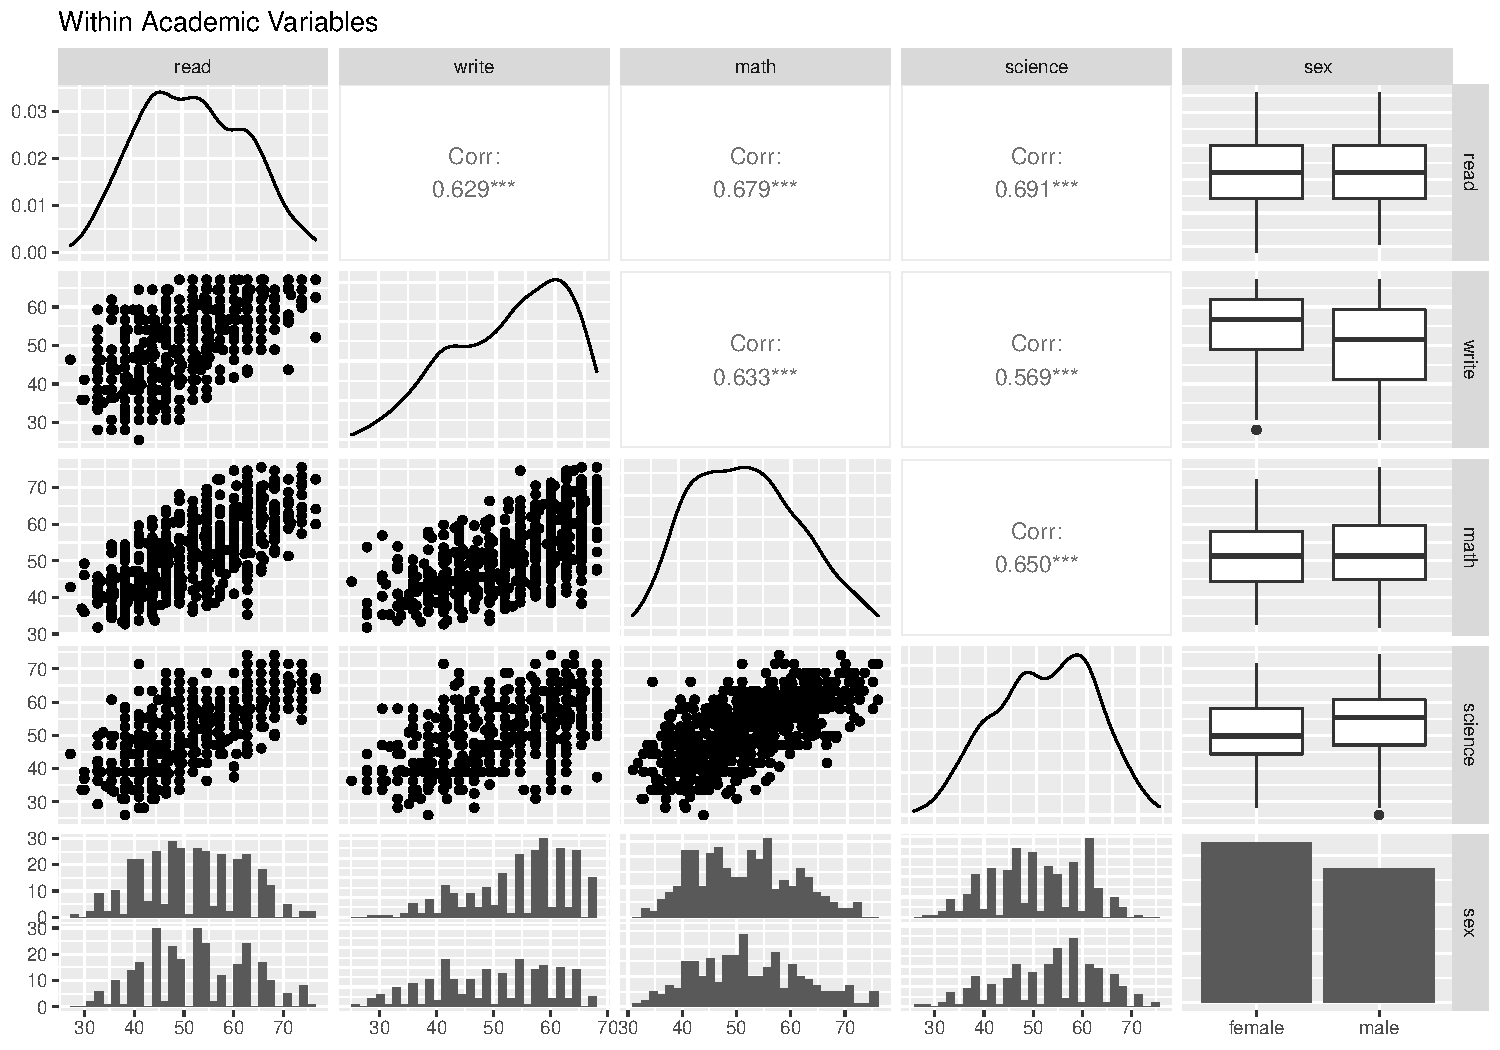
\includegraphics{claseIntro_practico12_final_files/figure-beamer/unnamed-chunk-19-1.pdf}

\normalsize
\end{frame}

\begin{frame}{Filogenética: librería ggtree}
\protect\hypertarget{filogenuxe9tica-libreruxeda-ggtree}{}
\small

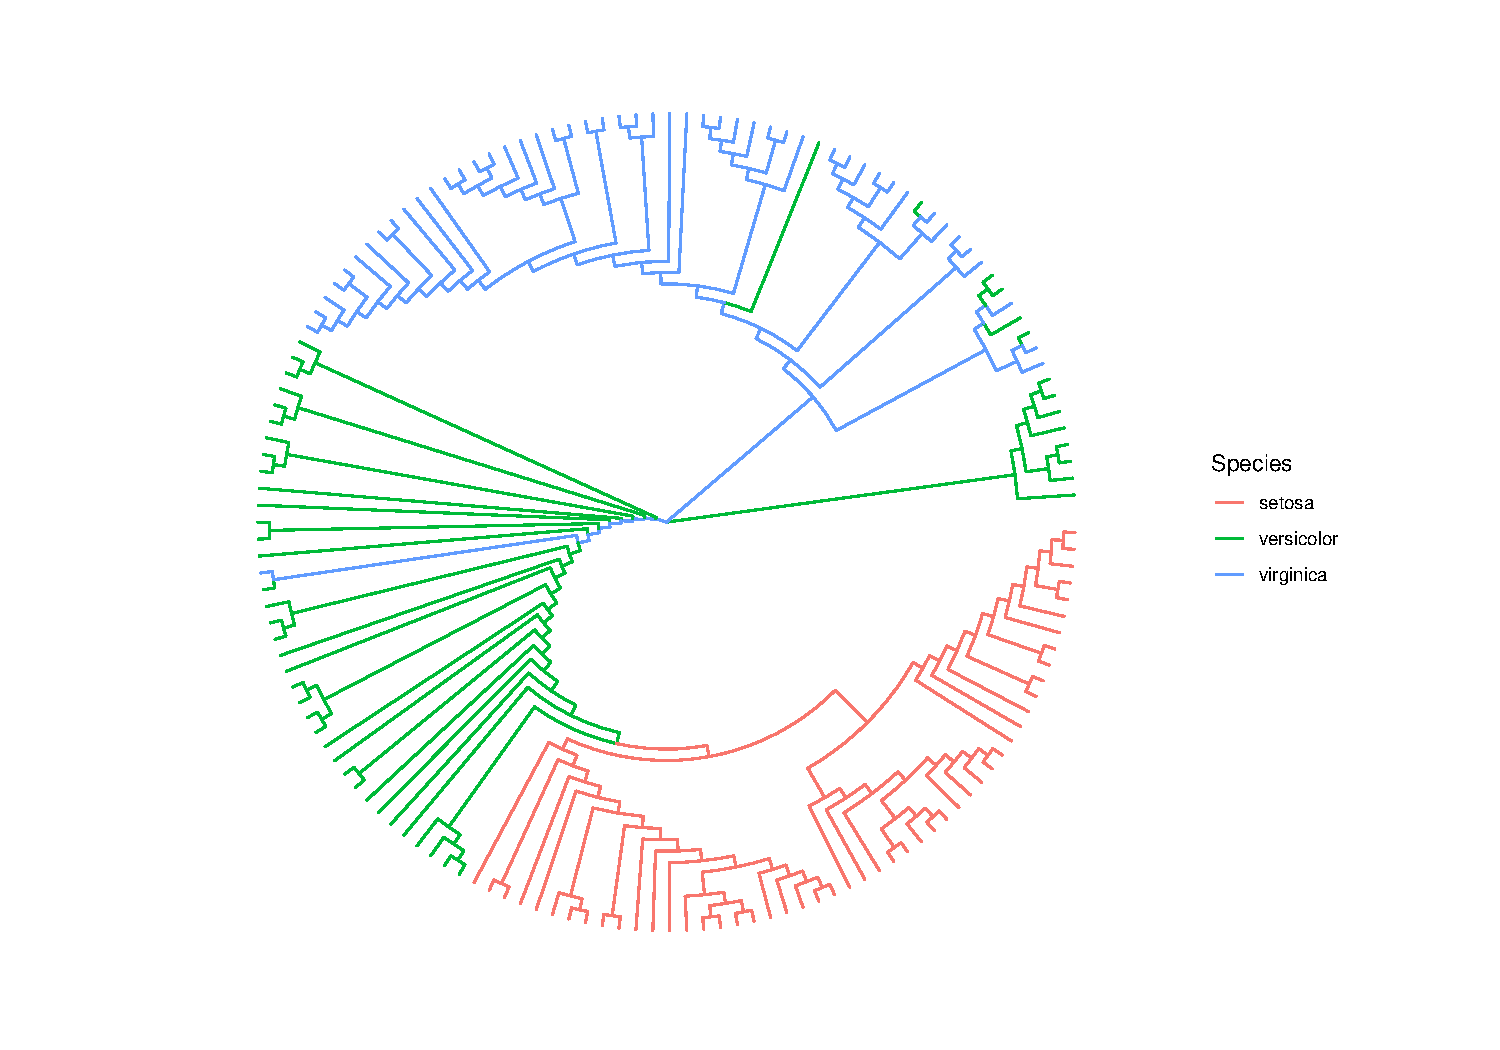
\includegraphics{claseIntro_practico12_final_files/figure-beamer/unnamed-chunk-20-1.pdf}

\normalsize
\end{frame}

\begin{frame}{Genómica: BioCircos/\textbf{rcirclize} y gggnomics, ggbio}
\protect\hypertarget{genuxf3mica-biocircosrcirclize-y-gggnomics-ggbio}{}
\begin{center}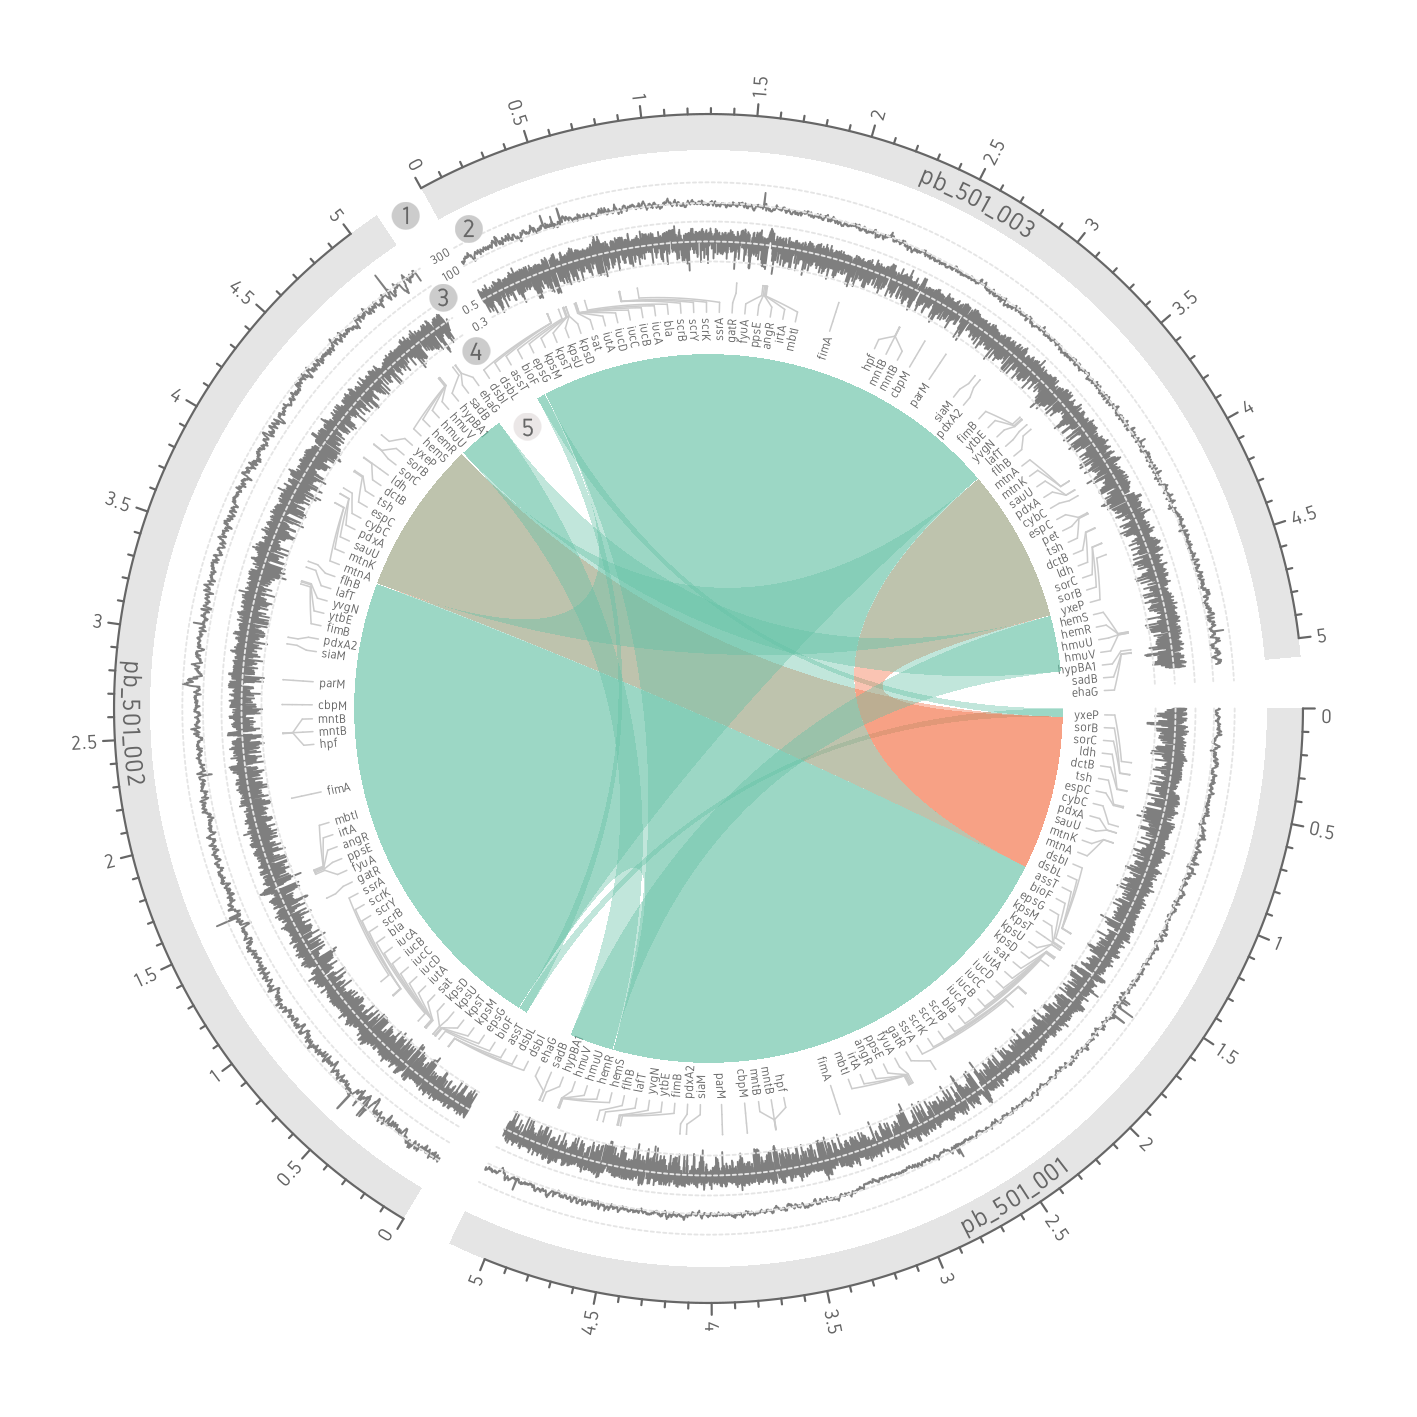
\includegraphics[width=0.7\linewidth]{../../imgs/rcirclize} \end{center}
\end{frame}

\begin{frame}{Genómica: BioCircos/rcirclize y gggnomics, \textbf{ggbio}}
\protect\hypertarget{genuxf3mica-biocircosrcirclize-y-gggnomics-ggbio-1}{}
\begin{center}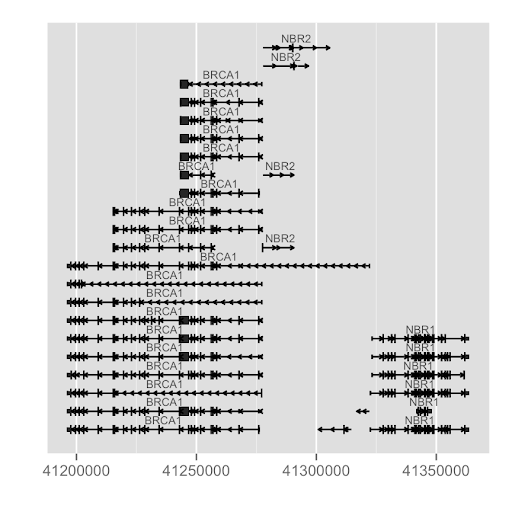
\includegraphics[width=0.7\linewidth]{../../imgs/ggnomics_1} \end{center}
\end{frame}

\begin{frame}{Genómica: BioCircos/rcirclize y gggnomics, \textbf{ggbio}}
\protect\hypertarget{genuxf3mica-biocircosrcirclize-y-gggnomics-ggbio-2}{}
\begin{center}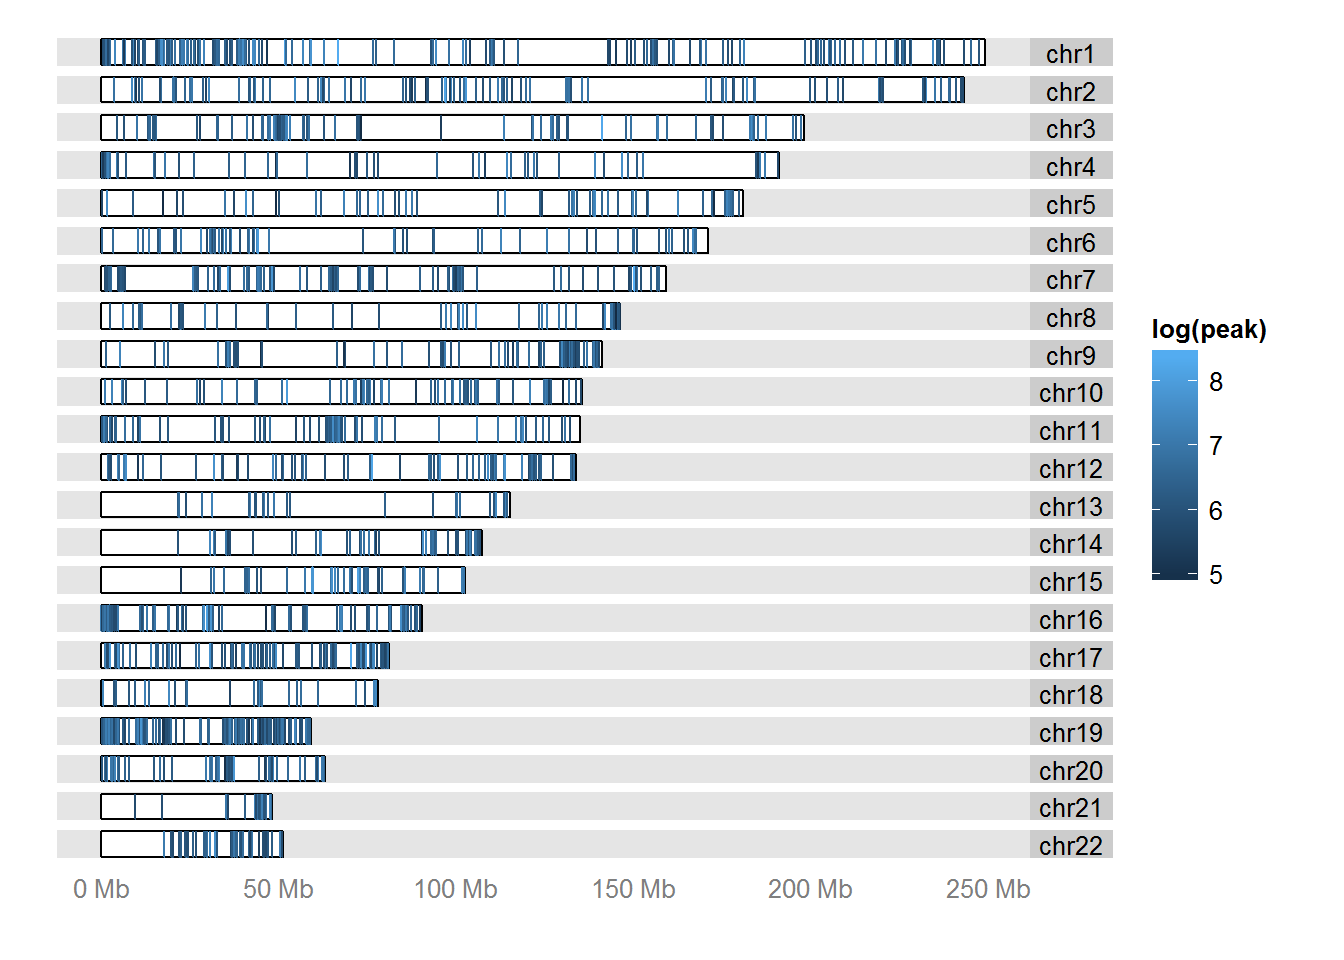
\includegraphics[width=0.95\linewidth]{../../imgs/ggnomics_2} \end{center}
\end{frame}

\hypertarget{lugares-interesantes-para-leer}{%
\section{Lugares interesantes para
leer}\label{lugares-interesantes-para-leer}}

\begin{frame}{¿Donde encuentro info sobre estos paquetes?}
\protect\hypertarget{donde-encuentro-info-sobre-estos-paquetes}{}
\begin{center}
\includegraphics[width=0.45\linewidth]{../../imgs/cover_rfordatascience} \end{center}

La mejor puerta de entrada al universo \emph{tidyverse} (y a buena parte
de \emph{R}!)
\end{frame}

\begin{frame}{¿Donde encuentro info sobre estos paquetes?}
\protect\hypertarget{donde-encuentro-info-sobre-estos-paquetes-1}{}
\begin{itemize}
\item
  \emph{Cheatsheets} y \emph{Vignettes} de las librerias \vspace{10pt}
\item
  \emph{From Data to Viz} \href{https://www.data-to-viz.com/}{(link)}:
  una buena pagina para ver como se hacen algunos graficos especificos
  \vspace{10pt}
\item
  Paginas con cursos cortos, en especial: \vspace{10pt}

  \begin{itemize}
  \tightlist
  \item
    \emph{Software carpentry}
    \href{https://software-carpentry.org/}{(link)}, con cursos en ingles
    y espanhol \vspace{5pt}
  \item
    \emph{Our coding club}
    \href{https://ourcodingclub.github.io/}{(link)}, de un grupo de
    ecologia de Escocia \vspace{10pt}
  \end{itemize}
\item
  Papers del grupo de Hadley Wickham (creador de tidyverse).

  \begin{itemize}
  \tightlist
  \item
    Estan bastante a la mano (no son de programacion pura y dura), y
    ayudan a entender la logica de fondo \vspace{10pt}
  \item
    Paper sobre \emph{Tidy data}
    (\href{https://vita.had.co.nz/papers/tidy-data.pdf}{link})
    \vspace{5pt}
  \item
    Paper sobre \emph{Layered grammar of graphics}
    (\href{https://byrneslab.net/classes/biol607/readings/wickham_layered-grammar.pdf}{link})
  \end{itemize}
\end{itemize}
\end{frame}

\end{document}
